\chapter{Ingénierie des exigences}
\section{Approche Top-Down}

Dans cette partie nous allons analyser notre système avec une approche Top-Down. Cela signifie que nous adopterons une démarche de conception descendante. Pour cela nous avons tracé le diagramme "bête à cornes", que l'on peut voir sur la figure \ref{fig:beteacorne}. Il permet de représenter graphiquement l'expression du besoin. Comme on peut le voir sur le diagramme, le système BMONS rend service aux apiculteurs en agissant sur une ou plusieurs ruches. Il a pour but d'aider la surveillance d'un rucher et d'avertir l'apiculteur en cas de problème.

\clearpage

\begin{figure}[h!]
\centering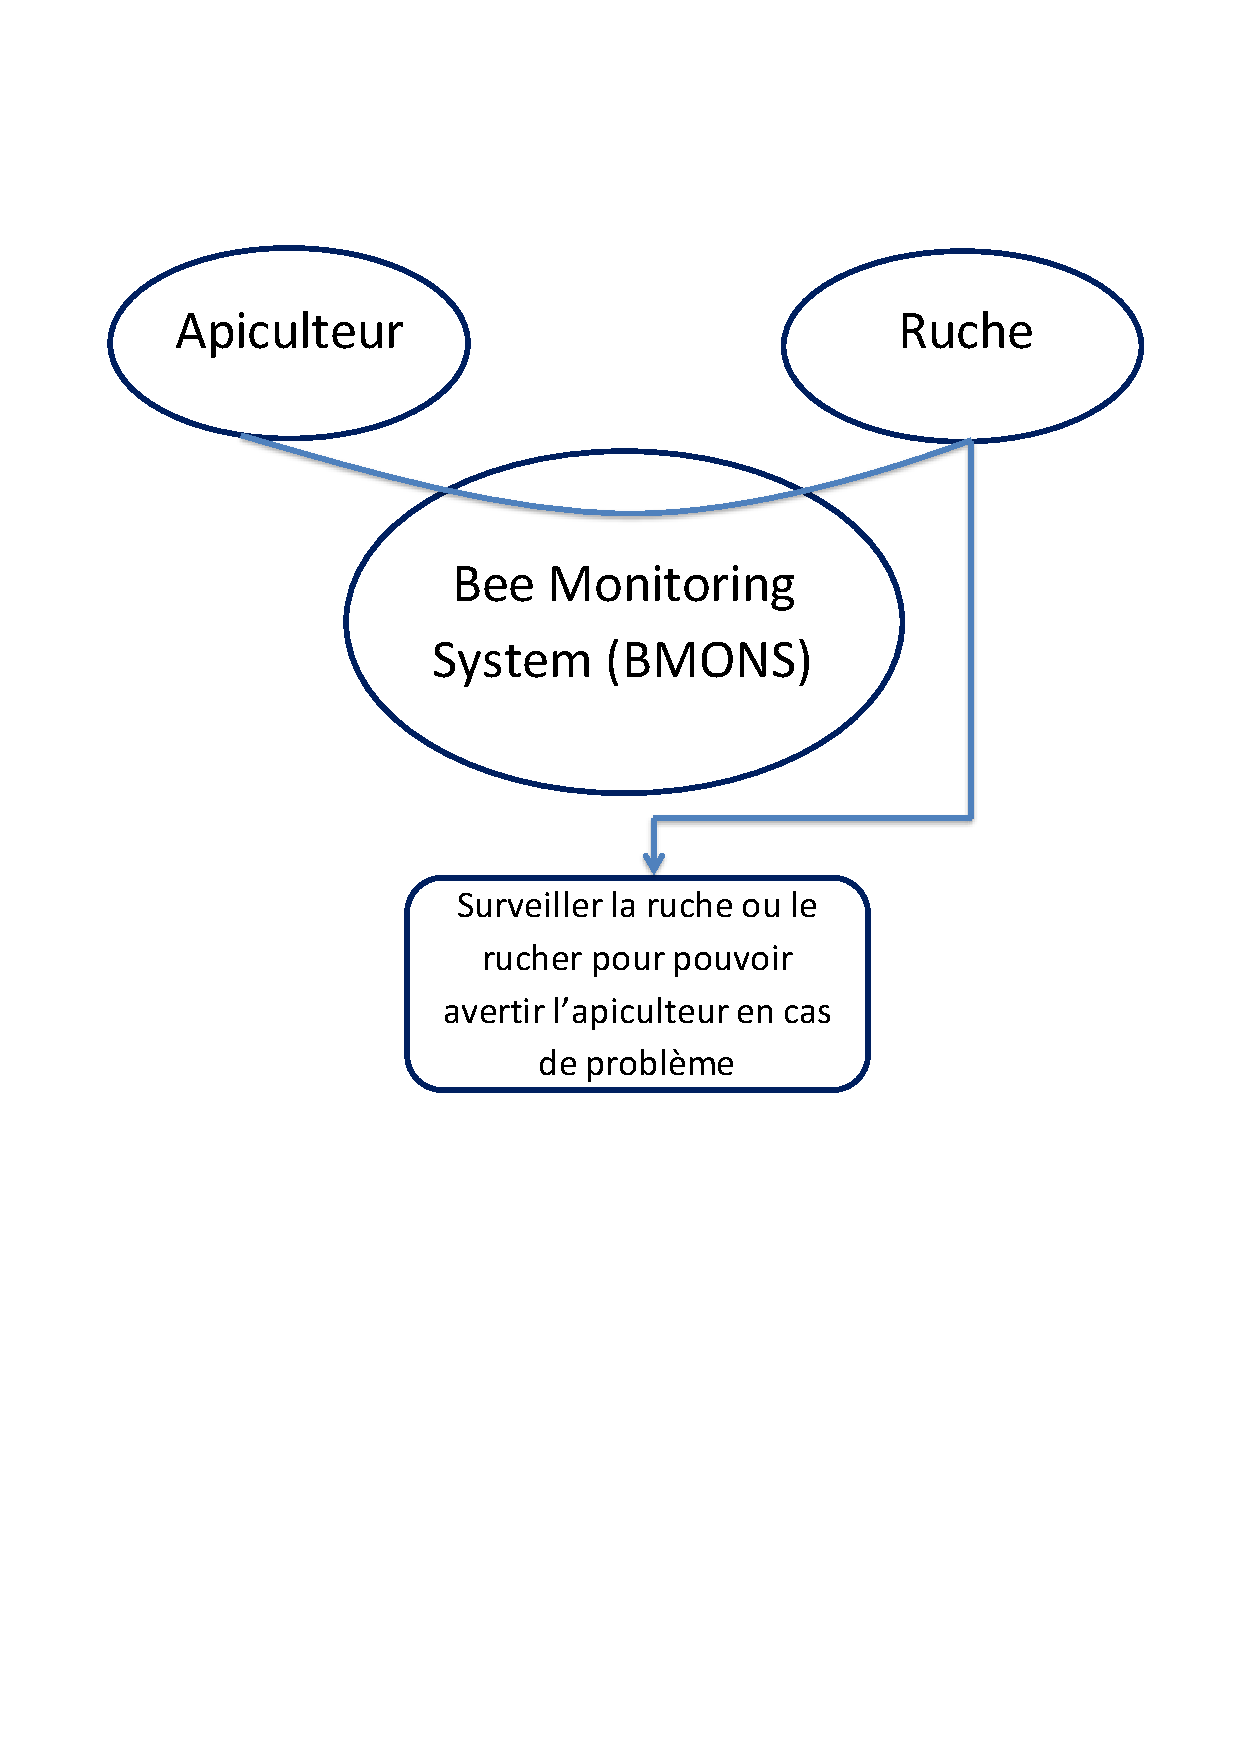
\includegraphics[scale=0.7]{BeteACornesBMONS.pdf}
\caption{\label{fig:beteacorne} Diagramme "bête à cornes" du système BMONS}
\end{figure}


\section{Approche Bottom-Up}

\section{Fonctions principales du système}

Les fonctions principale, services et contraintes du système sont regroupées dans ce diagramme pieuvre, figure \ref{fig:diagpieuvre}. Les buts et les contraintes imposées au système y sont également représentés. 
 
\begin{figure}[h]
\centering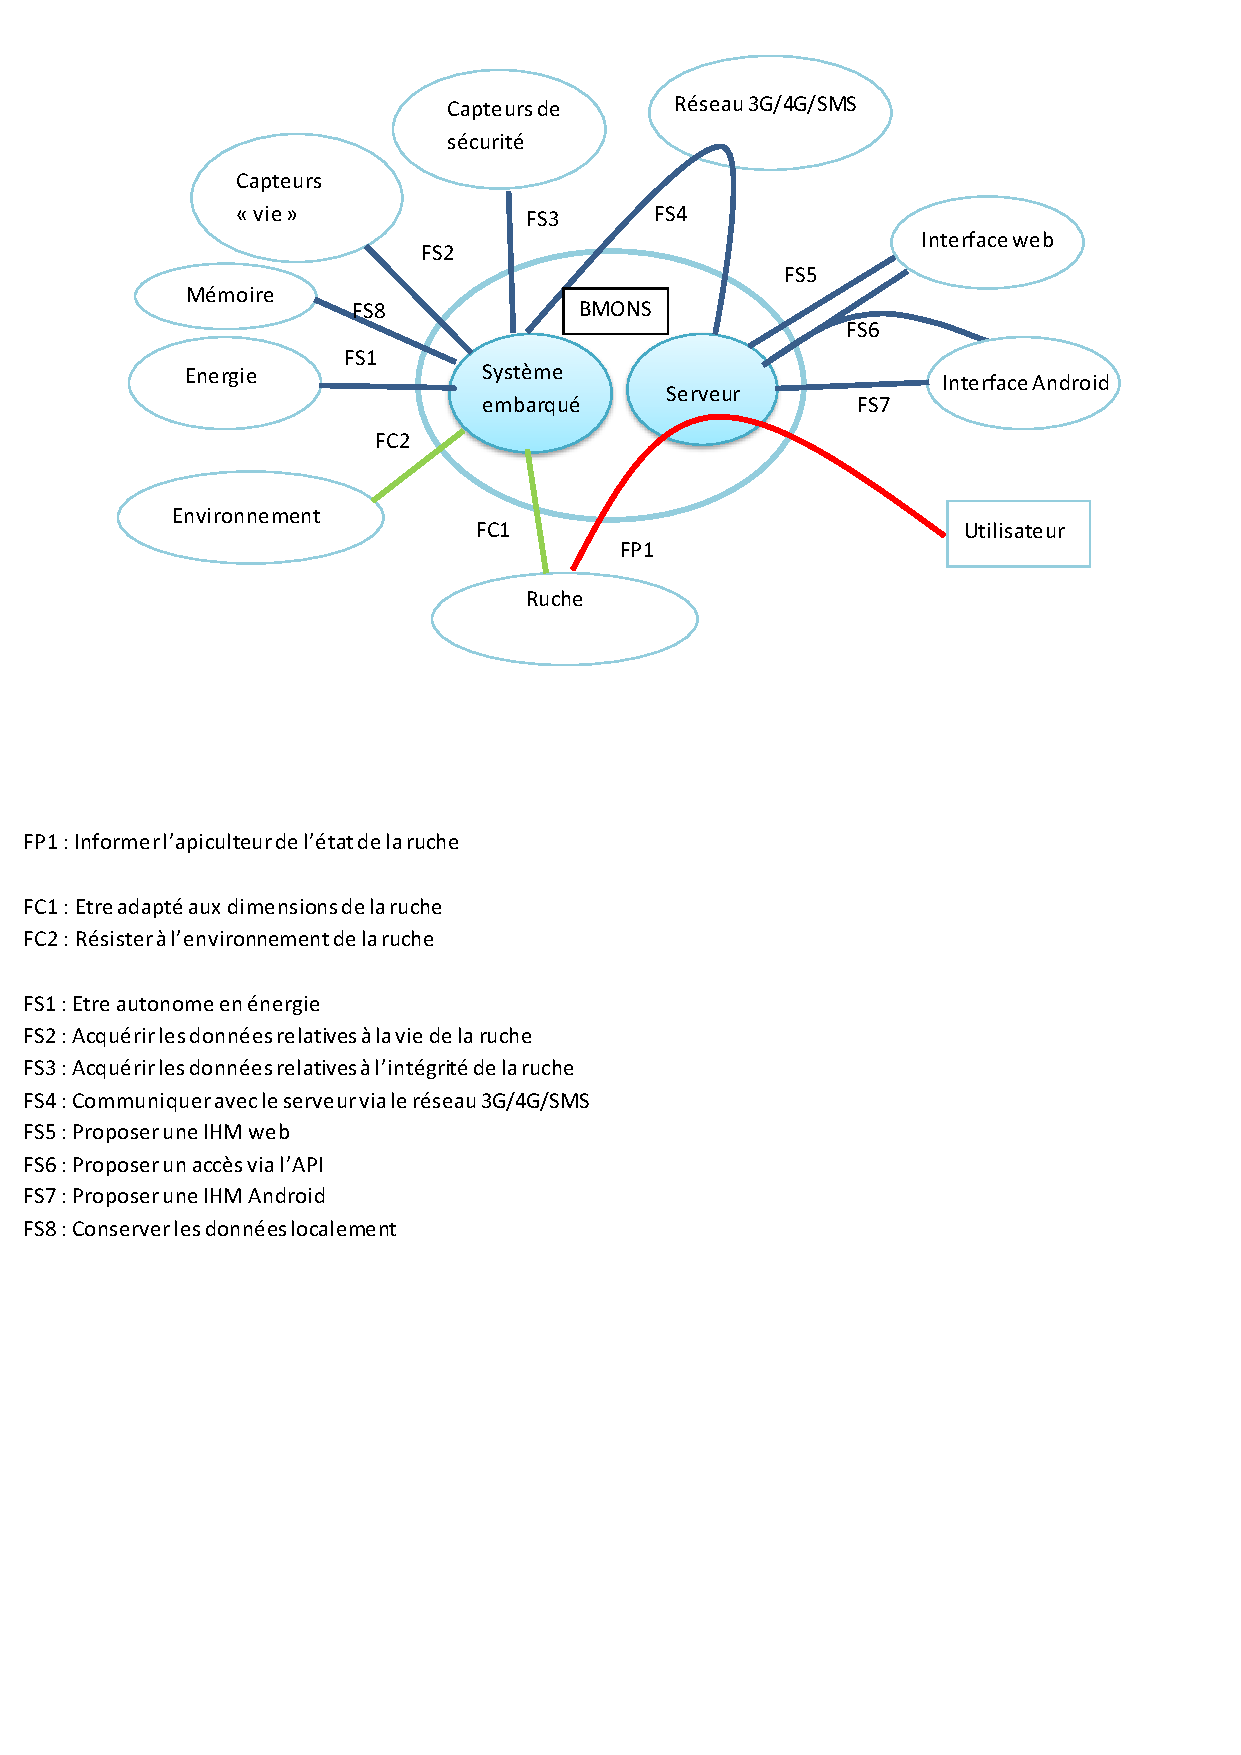
\includegraphics[scale=0.7]{diagpieuvre.pdf}
\caption{\label{fig:diagpieuvre} Diagramme pieuvre de système BMONS}
\end{figure}


\chapter{Spécification fonctionnelle  3 axes}

\section{Raffinement FAST}
Le diagramme FAST regroupe les fonctions principales, techniques et contraintes globales définies dans lors de 
l'établissement des exigences et après leur discussion avec le client. Leur raffinement en sous fonctions et les solutions techniques 
associées a celles-ci apparaissent également. Il a évolué au cours du projet en fonction des autres documents 
d'ingénierie système et des solutions techniques retenues. On peut voir la version finale du FAST sur la figure \ref{fig:fast}

\clearpage

\begin{figure}[h!]
\centering\includegraphics[scale=0.7]{FAST_BMONS.pdf}
\caption{\label{fig:fast} Diagramme FAST du système BMONS}
\end{figure}


\section{Spécification des données}
La spécification des données permet de mettre à jour les différentes grandeurs 
et unités intervenant dans notre système. Grâce à cela, nous savons exactement 
quel type donnée traiter et envoyer à l'apiculteur et/ou au serveur en fonction des évènements. Cette étude a aussi permis d'établir les alertes qu'il va falloir prévoir afin d'avertir le propriétaire de l'état de son rucher. 

!!!  image de spécification des données  !!!

\section{Spécification des comportements}

Nous allons ici décrire le fonctionnement de notre système. Il est résumé dans la figure \ref{fig:sp_comp}.

\begin{figure}[h!]
\centering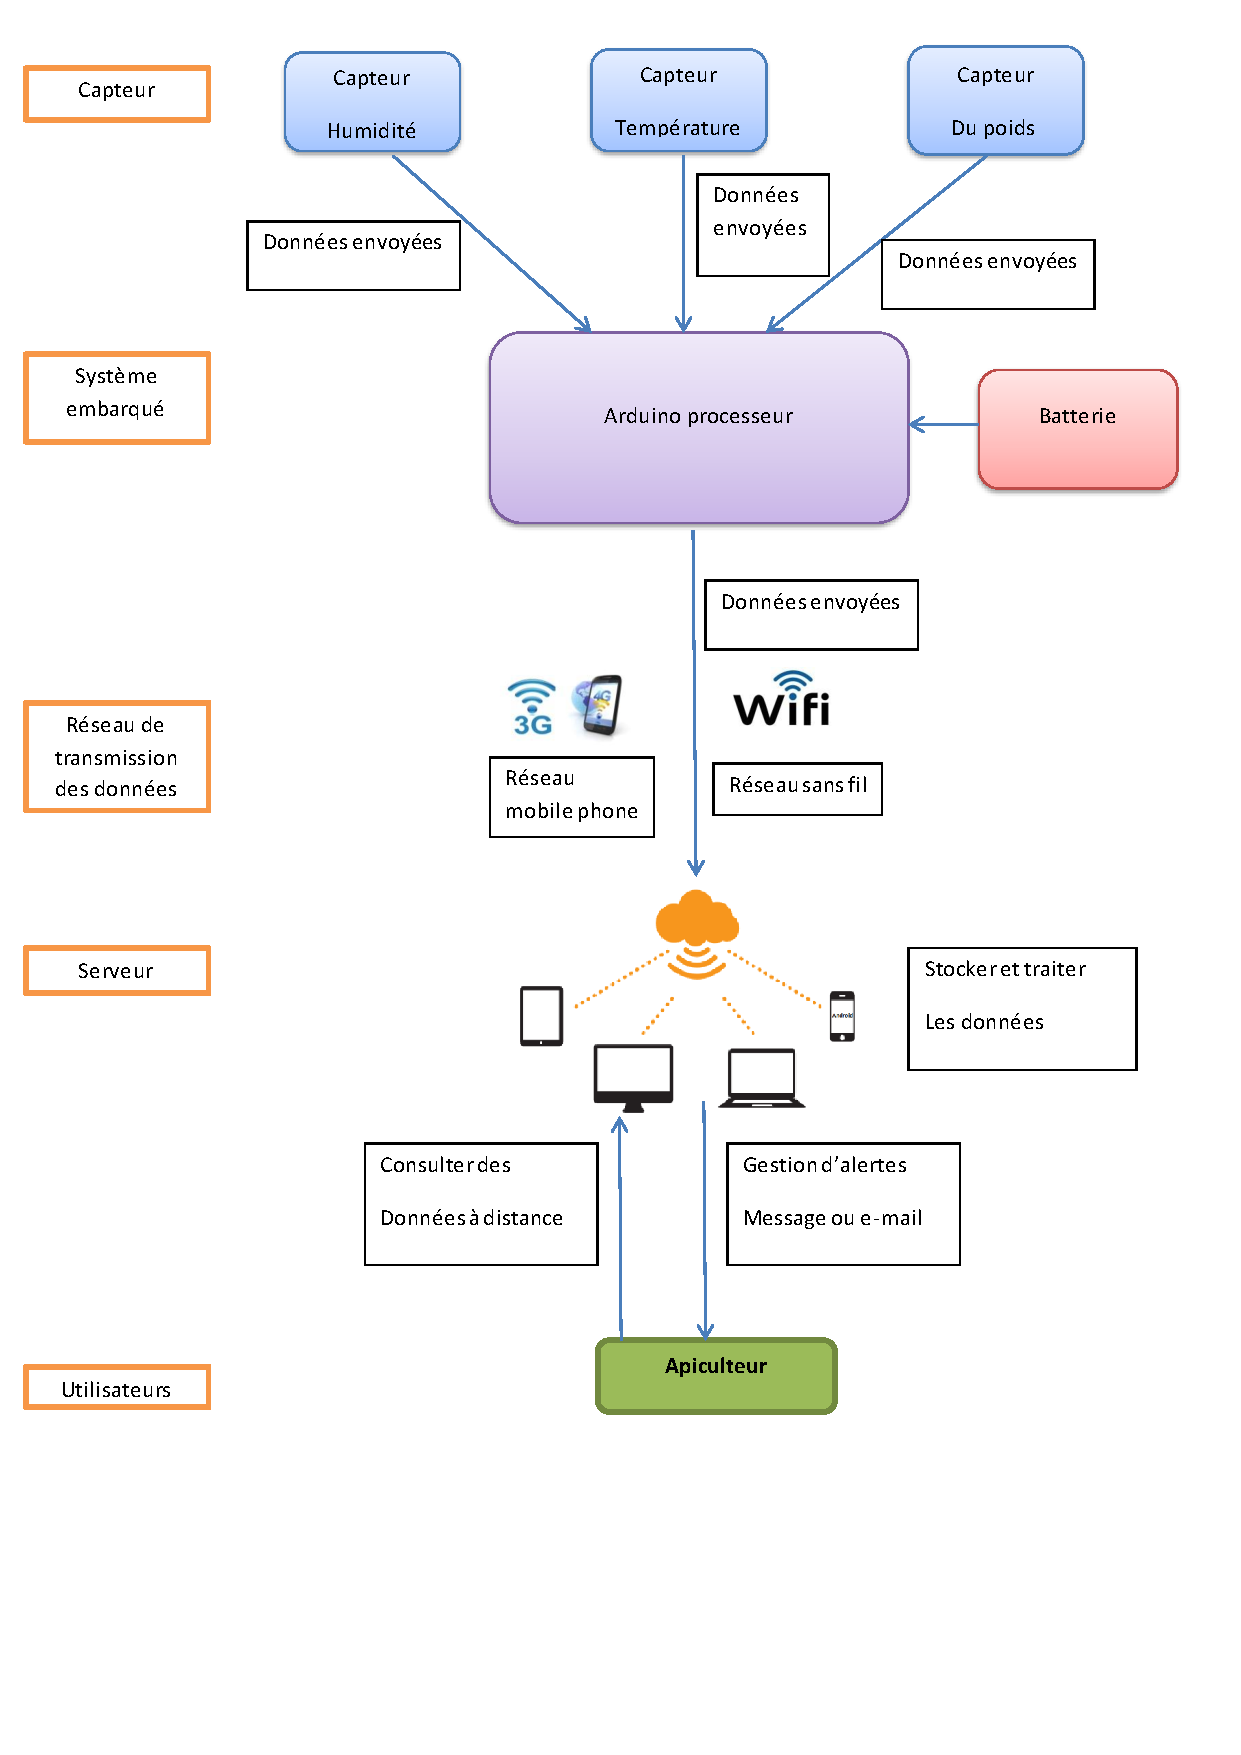
\includegraphics[scale=0.7]{specif_comp.pdf}
\caption{\label{fig:sp_comp} Diagramme de spécification des comportements}
\end{figure}

Les capteurs mesurent plusieurs paramètres internes à la ruche : l'humidité, la température et le poids de la ruche. Les données sont ensuite transmises au système embarqué. Dès que le système embarqué les reçoit, il traite les données, sélectionne celles qui sont valides et les envoi au serveur soit par le réseau sans fil (2G ou 3G), soit par le réseau téléphone si besoin. Une fois que le serveur reçoit les données, elles sont traitées et stockées dans une base de données sécurisée. Une représentation sous forme de graphiques permet une vision pratique et exploitable des informations par l'apiculteur.

Quand les mesures effectuées dépassent certain critères, par exemple, si la température est plus élevée que la température maximum pour la ruche, le serveur va générer un alerte qui sera envoyée à l'utilisateur, c’est-à-dire l'apiculteur, par SMS ou par e-mail. Par ailleurs, les apiculteurs peuvent consulter l’état de la ruche à distance afin de bien gérer la productivité de la ruche ou de limiter les situations problématiques. 

\pagebreak

\chapter{Architecture fonctionnelle}

L'étude de la spécification fonctionnelle trois axes a permis d'établir l'architecture fonctionnelle du système qui est représentée sur la figure \ref{fig:anaFonc}.
Ce schéma résume les interactions entre chaque partie: Bee Monitor qui regroupe l'ensemble des capteurs, la carte Arduino ainsi que la carte SSD pour l'enregistrement local des données, le module de transmission et le système d'alimentation rendant notre projet autonome en énergie. Chaque acteur interagissant avec le système y sont également représentés. 
  

\begin{figure}[h]
\centering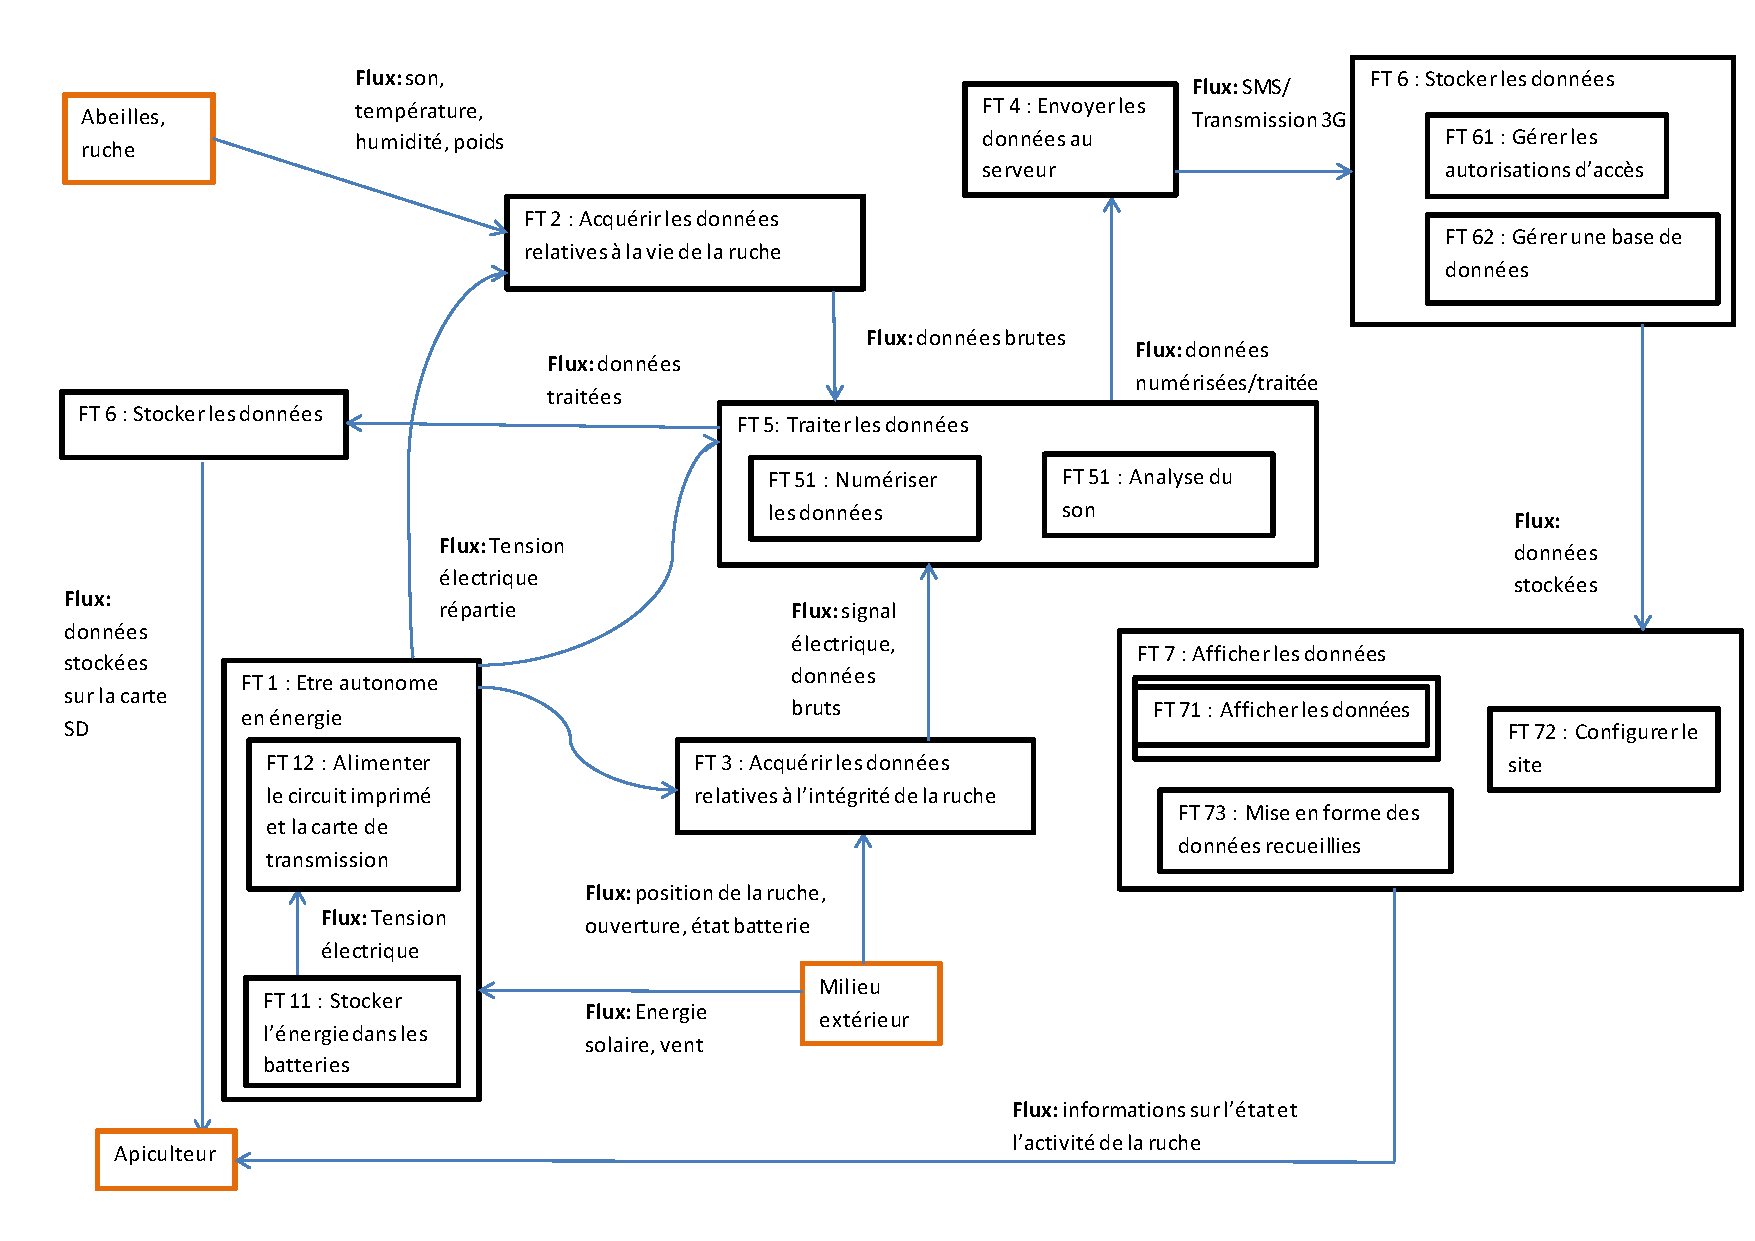
\includegraphics[scale=0.7]{analyseFonctionelle.pdf}
\caption{\label{fig:anaFonc} Architecture fonctionnelle}
\end{figure}    

